% file: 3-11-matchings-factors/chinese-postman-problem-decompose.tex

\documentclass[tikz]{standalone}
\usetikzlibrary{positioning, chains}

\begin{document}
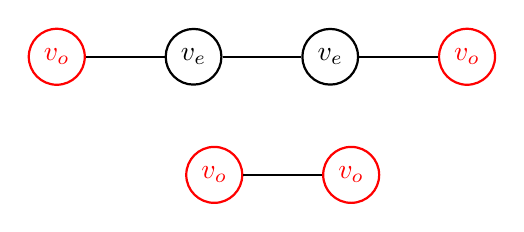
\begin{tikzpicture}[every node/.style = {draw, thick, circle, minimum size = 15pt},
  node distance = 1.0cm, every join/.style = {thick, -},
  start chain = 1 going right,
  start chain = 2 going right]
    \node [on chain = 1, join, red] {$v_o$};
    \node [on chain = 1, join] {$v_e$};
    \node [on chain = 1, join] {$v_e$};
    \node [on chain = 1, join, red] {$v_o$};

    \begin{scope}[xshift = 2.0cm, yshift = -1.5cm]
      \node [on chain = 2, join, red] {$v_o$};
      \node [on chain = 2, join, red] {$v_o$};
    \end{scope}
  \end{tikzpicture}
\end{document}
